\documentclass{article}
\usepackage[utf8]{inputenc}
\usepackage{graphicx}
\usepackage[dvipsnames]{xcolor}
\definecolor{amethyst}{rgb}{0.6, 0.4, 0.8}
\title{Reservation des salles}
\author{Mohammed AL JADD}
\date{2020 Avril}
\begin{document}
\maketitle

    




\includegraphics[width=\textwidth]{img/Go.png}

\begin{enumerate}
    
     \item  \textcolor{red}{\huge Introduction} : 
     \vspace{1cm}
 
   \setlength{\parindent}{1cm} Mon projet est une application web , sous le nom Réservation des salles à distance, qui répondra aux problématiques suivantes:
   \begin{itemize}
     
        \item Difficulté à trouver une salle disponible.
        \item Le professeur a besoin d'être dans l'institut pour trouver une salle disponible.
        \item L'emploi du temps doit être modifié chaque fois qu'il n'y a pas de salle disponible.
        
            Les langages de programmation que j'ai utilisés dans mon projet : \textcolor{blue}{ \textbf{HTML}},\textcolor{blue}{\textbf{CSS}},\textcolor{blue}{\textbf{JavaScript}} et \textcolor{blue}{\textbf{PHP}}.
   \end{itemize}
   
   Il m'a fallu environ deux mois pour terminer ce projet. J'ai commencé en février et terminé en avril.\par Ce projet m'a permis d'apprendre à travailler avec github et à écrire du code long en \textcolor{blue}{\textbf{PHP}}, \textcolor{blue}{\textbf{CSS}} et \textcolor{blue}{\textbf{JavaScript}}. De plus, comme j'ai appris certaines commandes \textcolor{blue}{\textbf{GITHUB}}, cela me permettra à l'avenir de collaborer avec d'autres peuples, même à la maison.\par l'une des choses importantes que le projet me fournit est de savoir comment gérer votre projet et le discrétiser en étapes pour faciliter son progression.\par Pour \textcolor{blue}{\textbf{GITHUB}}, la meilleure chose que j'ai aimé est que vous ne serez pas attiré par votre machie puisque votre projet est stocké en ligne.
   
   
   
   
   
   
   \item \textcolor{red}{\huge L'avancement du projet} :
   
    Ci-dessous, je vais expliquer chaque tâche en détail:
        
        \begin{enumerate}
        \item \textcolor{amethyst}{Apprenez le langage de programmation php}:
        
        \vspace{0.4cm}
            \setlength{\parindent}{1cm} J'ai appris la langage de programmation PHP parce que dans la plupart du temps je vais interagir avec la base de données.
            J'ai suivi des cours PHP sur une chaîne YouTube s'appelle mmtuts en regardant des petites videos.     
            
        \item \textcolor{amethyst}{Déterminer les pages que le site Web contiendra}.
            
            \vspace{0.4cm}
                \setlength{\parindent}{1cm} La détermination des pages est une étape très importante car elle vous donne une vision globale de votre website.L'image suivante montre toutes les pages de notre site Web et montre également les redirections entre elles.
                
               \vspace{0.6cm}
               \hspace*{-1.05in}
               \noindent\makebox[\textwidth]{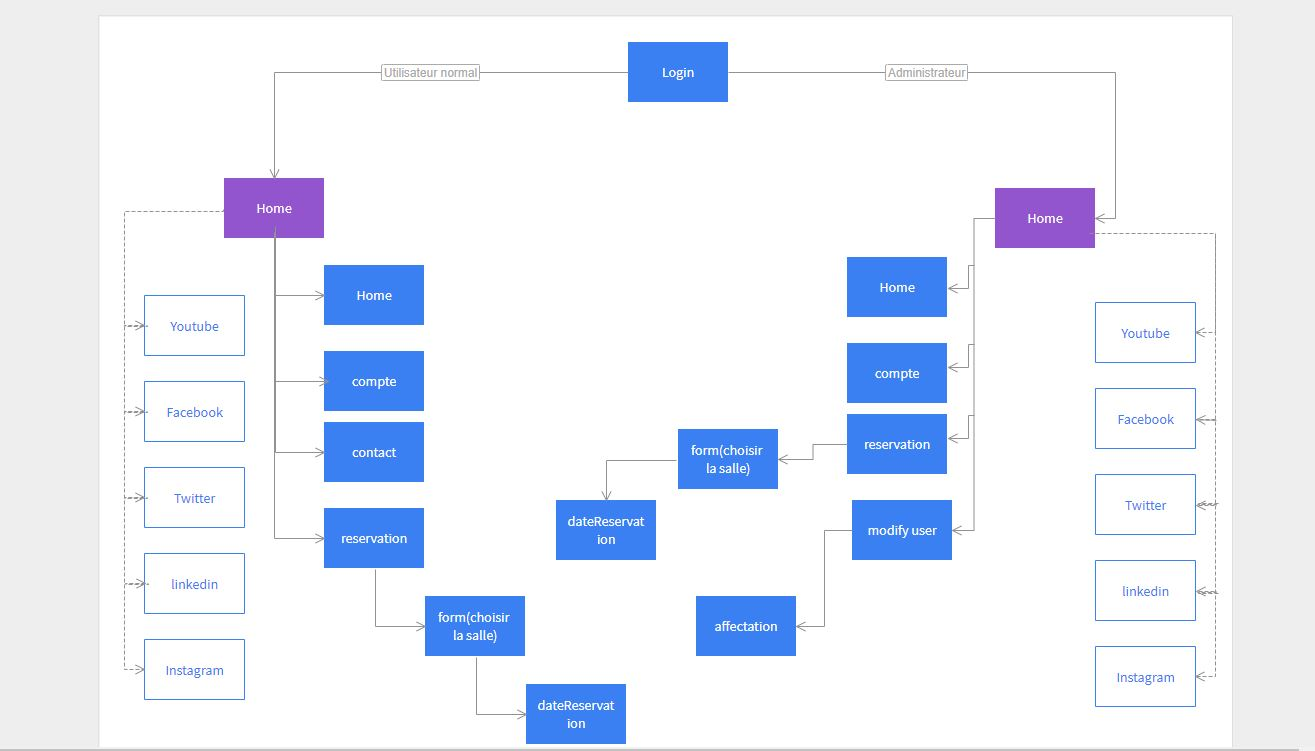
\includegraphics[width=\paperwidth,height=12cm]{img/map.jpg}}
                \vspace{0.6cm}
                 \item \textcolor{amethyst}{Installation de la base de données}.
           \vspace{0.4cm}
           
           
            \setlength{\parindent}{1cm}  J'ai installer logiciel xampp. Ce permet de mettre en place un serveur Web local et un serveur de Base de donnée. Après avoir réalisé le modèle entité-association, j'ai créé ma base de données qui est présentée dans l'image suivante :
            
            
            
            \hspace*{-1.05in}
               \noindent\makebox[\textwidth]{\includegraphics[width=\paperwidth,height=12cm]{img/dataBase.png}}
        
        
         \item \textcolor{amethyst}{Créer des maquettes}.
         
         \vspace{0.4cm}
                \setlength{\parindent}{1cm} J'ai créé des maquettes pour mon site Web en utilisant le site Web moqups.com. Ils sont présentés dans le dossier maquettes.
         
         \item \textcolor{amethyst}{Apprenez \textbf{GITHUB}}.
         
         \vspace{0.4cm}
                \setlength{\parindent}{1cm} J'ai regardé un video sur youtube pour apprendre comment commiter du VISUAL STUDIO CODE, créer un project basic-KANBAN.
         
         \item \textcolor{amethyst}{Créer des pages WEB}.
         
         \vspace{0.4cm}
                \setlength{\parindent}{1cm} J'ai commencé à créer des pages Web \textcolor{blue}{\textbf{PHP}} après que je termine une page je crée une page \textcolor{blue}{\textbf{CSS}} pour appliquer les style .Mais j'ai respecté la façon que les informations entre par l'utlisateur vont  être traitées dans des pages des différents. Par exemple utilisateur elle veut changer son mot de passe, son nouveau mot de passe va être traité dans une autre page.
         
         \hspace*{-1.05in}
               \noindent\makebox[\textwidth]{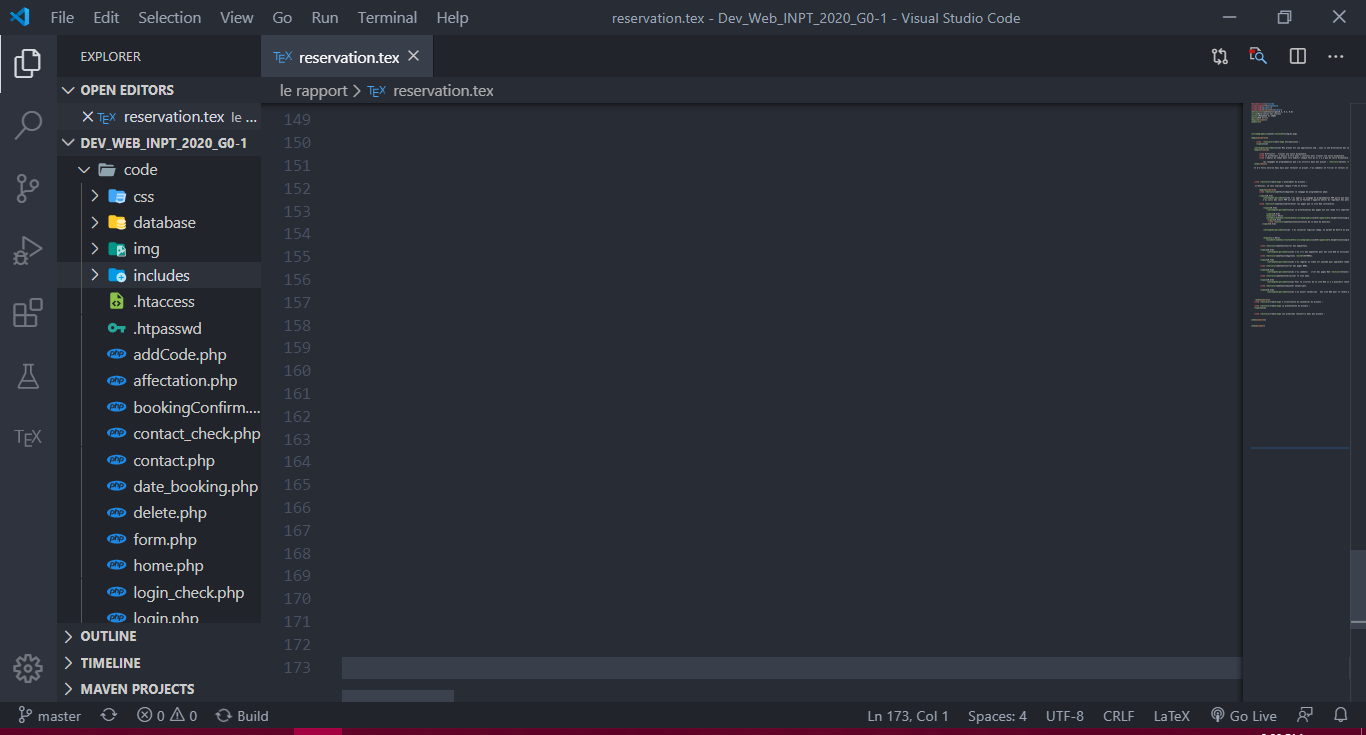
\includegraphics[width=\paperwidth,height=12cm]{img/visual.png}}
         \item \textcolor{amethyst}{Sécuriser le site web}.
         
         \vspace{0.4cm}
                \setlength{\parindent}{1cm} Pour la sécurité de ce site Web il y a plusieurs choses que j'ai fait la première chose est d'empêcher l'accès à certaines pages sans connexion. Une deuxième chose est d'empêcher l'accès à certains car ils sont destinés à l'administrateur même en cas de connexion.
         
         \item \textcolor{amethyst}{Ajouter JavaScript}.
         
         \vspace{0.4cm}
                \setlength{\parindent}{1cm} J'ai ajouté JavaScript à mon site Web pour le rendre plus dynamique, par exemple, lorsqu'il y a des erreurs comme si l'utilisateur n'a pas entré ses informations et soumis, le site Web affichera une erreur indiquant que les fichiers sont vides à l'aide de la boîte d'alerte.
         
         
   
    \end{enumerate}
   \item \textcolor{red}{\huge L'illustration du calendrier du projet} :  
   
   \item \textcolor{red}{\huge La presentation du projet} :  
   \vspace{1cm}
   

   \item \textcolor{red}{\huge Les problèmes rencontrés dans mon projet} :
   
  
\end{enumerate}


\end{document}
